%%%%%%%%%%%%%%%%%%%%%%%%%%%%%%%%%%%%%%%%%
% Masters/Doctoral Thesis 
% LaTeX Template
% Version 2.5 (27/8/17)
%
% This template was downloaded from:
% http://www.LaTeXTemplates.com
%
% Version 2.x major modifications by:
% Vel (vel@latextemplates.com)
%
% This template is based on a template by:
% Steve Gunn (http://users.ecs.soton.ac.uk/srg/softwaretools/document/templates/)
% Sunil Patel (http://www.sunilpatel.co.uk/thesis-template/)
%
% Template license:
% CC BY-NC-SA 3.0 (http://creativecommons.org/licenses/by-nc-sa/3.0/)
%
%%%%%%%%%%%%%%%%%%%%%%%%%%%%%%%%%%%%%%%%%

%----------------------------------------------------------------------------------------
%	PACKAGES AND OTHER DOCUMENT CONFIGURATIONS
%----------------------------------------------------------------------------------------

\documentclass[
11pt, % The default document font size, options: 10pt, 11pt, 12pt
%oneside, % Two side (alternating margins) for binding by default, uncomment to switch to one side
english, % ngerman for German
singlespacing, % Single line spacing, alternatives: onehalfspacing or doublespacing
%draft, % Uncomment to enable draft mode (no pictures, no links, overfull hboxes indicated)
%nolistspacing, % If the document is onehalfspacing or doublespacing, uncomment this to set spacing in lists to single
%liststotoc, % Uncomment to add the list of figures/tables/etc to the table of contents
%toctotoc, % Uncomment to add the main table of contents to the table of contents
%parskip, % Uncomment to add space between paragraphs
%nohyperref, % Uncomment to not load the hyperref package
headsepline, % Uncomment to get a line under the header
%chapterinoneline, % Uncomment to place the chapter title next to the number on one line
%consistentlayout, % Uncomment to change the layout of the declaration, abstract and acknowledgements pages to match the default layout
]{MastersDoctoralThesis} % The class file specifying the document structure

\usepackage[utf8]{inputenc} % Required for inputting international characters
\usepackage[T1]{fontenc} % Output font encoding for international characters

\usepackage{mathpazo} % Use the Palatino font by default

\usepackage[backend=bibtex,style=authoryear,natbib=true]{biblatex} % Use the bibtex backend with the authoryear citation style (which resembles APA)

\addbibresource{example.bib} % The filename of the bibliography

\usepackage[autostyle=true]{csquotes} % Required to generate language-dependent quotes in the bibliography

\usepackage{mathtools} % We need to use mathematical symbols
\usepackage{amsfonts} % We need to use mathbb
\usepackage{algorithm}
\usepackage[]{algpseudocode}


\makeatletter
\def\BState{\State\hskip-\ALG@thistlm}
\makeatother

%----------------------------------------------------------------------------------------
%	MARGIN SETTINGS
%----------------------------------------------------------------------------------------

\geometry{
	paper=a4paper, % Change to letterpaper for US letter
	inner=2.5cm, % Inner margin
	outer=3.8cm, % Outer margin
	bindingoffset=.5cm, % Binding offset
	top=1.5cm, % Top margin
	bottom=1.5cm, % Bottom margin
	%showframe, % Uncomment to show how the type block is set on the page
}

%----------------------------------------------------------------------------------------
%	THESIS INFORMATION
%----------------------------------------------------------------------------------------

\thesistitle{Practical zk-SNARKS} % Your thesis title, this is used in the title and abstract, print it elsewhere with \ttitle
\supervisor{Prof. Dr. Sr\'{d}an \v{C}apkun \textsc{Smith}} % Your supervisor's name, this is used in the title page, print it elsewhere with \supname
\examiner{} % Your examiner's name, this is not currently used anywhere in the template, print it elsewhere with \examname
\degree{MSc in Computer Science} % Your degree name, this is used in the title page and abstract, print it elsewhere with \degreename
\author{Uro\v{s} Te\v{s}i\'{c}} % Your name, this is used in the title page and abstract, print it elsewhere with \authorname
\addresses{} % Your address, this is not currently used anywhere in the template, print it elsewhere with \addressname

\subject{Computer Science} % Your subject area, this is not currently used anywhere in the template, print it elsewhere with \subjectname
\keywords{} % Keywords for your thesis, this is not currently used anywhere in the template, print it elsewhere with \keywordnames
\university{\href{http://www.ethz.ch}{University Name}} % Your university's name and URL, this is used in the title page and abstract, print it elsewhere with \univname
\department{\href{http://department.university.com}{D-INFK}} % Your department's name and URL, this is used in the title page and abstract, print it elsewhere with \deptname
\group{\href{http://researchgroup.university.com}{System Security Group}} % Your research group's name and URL, this is used in the title page, print it elsewhere with \groupname
\faculty{\href{http://faculty.university.com}{Faculty Name}} % Your faculty's name and URL, this is used in the title page and abstract, print it elsewhere with \facname

\AtBeginDocument{
\hypersetup{pdftitle=\ttitle} % Set the PDF's title to your title
\hypersetup{pdfauthor=\authorname} % Set the PDF's author to your name
\hypersetup{pdfkeywords=\keywordnames} % Set the PDF's keywords to your keywords
}

\begin{document}

\frontmatter % Use roman page numbering style (i, ii, iii, iv...) for the pre-content pages

\pagestyle{plain} % Default to the plain heading style until the thesis style is called for the body content

%----------------------------------------------------------------------------------------
%	TITLE PAGE
%----------------------------------------------------------------------------------------

\begin{titlepage}
\begin{center}

\vspace*{.06\textheight}
{\scshape\LARGE \univname\par}\vspace{1.5cm} % University name
\textsc{\Large Doctoral Thesis}\\[0.5cm] % Thesis type

\HRule \\[0.4cm] % Horizontal line
{\huge \bfseries \ttitle\par}\vspace{0.4cm} % Thesis title
\HRule \\[1.5cm] % Horizontal line
 
\begin{minipage}[t]{0.4\textwidth}
\begin{flushleft} \large
\emph{Author:}\\
\href{http://www.johnsmith.com}{\authorname} % Author name - remove the \href bracket to remove the link
\end{flushleft}
\end{minipage}
\begin{minipage}[t]{0.4\textwidth}
\begin{flushright} \large
\emph{Supervisor:} \\
\href{http://www.jamessmith.com}{\supname} % Supervisor name - remove the \href bracket to remove the link  
\end{flushright}
\end{minipage}\\[3cm]
 
\vfill

\large \textit{A thesis submitted in fulfillment of the requirements\\ for the degree of \degreename}\\[0.3cm] % University requirement text
\textit{in the}\\[0.4cm]
\groupname\\\deptname\\[2cm] % Research group name and department name
 
\vfill

{\large \today}\\[4cm] % Date
%\includegraphics{Logo} % University/department logo - uncomment to place it
 
\vfill
\end{center}
\end{titlepage}

%----------------------------------------------------------------------------------------
%	DECLARATION PAGE
%----------------------------------------------------------------------------------------

\begin{declaration}
\addchaptertocentry{\authorshipname} % Add the declaration to the table of contents
\noindent I, \authorname, declare that this thesis titled, \enquote{\ttitle} and the work presented in it are my own. I confirm that:

\begin{itemize} 
\item This work was done wholly or mainly while in candidature for a research degree at this University.
\item Where any part of this thesis has previously been submitted for a degree or any other qualification at this University or any other institution, this has been clearly stated.
\item Where I have consulted the published work of others, this is always clearly attributed.
\item Where I have quoted from the work of others, the source is always given. With the exception of such quotations, this thesis is entirely my own work.
\item I have acknowledged all main sources of help.
\item Where the thesis is based on work done by myself jointly with others, I have made clear exactly what was done by others and what I have contributed myself.\\
\end{itemize}
 
\noindent Signed:\\
\rule[0.5em]{25em}{0.5pt} % This prints a line for the signature
 
\noindent Date:\\
\rule[0.5em]{25em}{0.5pt} % This prints a line to write the date
\end{declaration}

\cleardoublepage

%----------------------------------------------------------------------------------------
%	QUOTATION PAGE
%----------------------------------------------------------------------------------------

\vspace*{0.2\textheight}

\noindent\enquote{\itshape Thanks to my solid academic training, today I can write hundreds of words on virtually any topic without possessing a shred of information, which is how I got a good job in journalism.}\bigbreak

\hfill Dave Barry

%----------------------------------------------------------------------------------------
%	ABSTRACT PAGE
%----------------------------------------------------------------------------------------

\begin{abstract}
\addchaptertocentry{\abstractname} % Add the abstract to the table of contents
The Thesis Abstract is written here (and usually kept to just this page). The page is kept centered vertically so can expand into the blank space above the title too\ldots
\end{abstract}

%----------------------------------------------------------------------------------------
%	ACKNOWLEDGEMENTS
%----------------------------------------------------------------------------------------

\begin{acknowledgements}
\addchaptertocentry{\acknowledgementname} % Add the acknowledgements to the table of contents
The acknowledgments and the people to thank go here, don't forget to include your project advisor\ldots
\end{acknowledgements}

%----------------------------------------------------------------------------------------
%	LIST OF CONTENTS/FIGURES/TABLES PAGES
%----------------------------------------------------------------------------------------

\tableofcontents % Prints the main table of contents

\listoffigures % Prints the list of figures

\listoftables % Prints the list of tables

%----------------------------------------------------------------------------------------
%	ABBREVIATIONS
%----------------------------------------------------------------------------------------

\begin{abbreviations}{ll} % Include a list of abbreviations (a table of two columns)

\textbf{LAH} & \textbf{L}ist \textbf{A}bbreviations \textbf{H}ere\\
\textbf{WSF} & \textbf{W}hat (it) \textbf{S}tands \textbf{F}or\\

\end{abbreviations}

%----------------------------------------------------------------------------------------
%	PHYSICAL CONSTANTS/OTHER DEFINITIONS
%----------------------------------------------------------------------------------------

\begin{constants}{lr@{${}={}$}l} % The list of physical constants is a three column table

% The \SI{}{} command is provided by the siunitx package, see its documentation for instructions on how to use it

Speed of Light & $c_{0}$ & \SI{2.99792458e8}{\meter\per\second} (exact)\\
%Constant Name & $Symbol$ & $Constant Value$ with units\\

\end{constants}

%----------------------------------------------------------------------------------------
%	SYMBOLS
%----------------------------------------------------------------------------------------

\begin{symbols}{lll} % Include a list of Symbols (a three column table)

$a$ & distance & \si{\meter} \\
$P$ & power & \si{\watt} (\si{\joule\per\second}) \\
%Symbol & Name & Unit \\

\addlinespace % Gap to separate the Roman symbols from the Greek

$\omega$ & angular frequency & \si{\radian} \\

\end{symbols}

%----------------------------------------------------------------------------------------
%	DEDICATION
%----------------------------------------------------------------------------------------

\dedicatory{For/Dedicated to/To my\ldots} 

%----------------------------------------------------------------------------------------
%	THESIS CONTENT - CHAPTERS
%----------------------------------------------------------------------------------------

\mainmatter % Begin numeric (1,2,3...) page numbering

\pagestyle{thesis} % Return the page headers back to the "thesis" style

% Include the chapters of the thesis as separate files from the Chapters folder
% Uncomment the lines as you write the chapters

% Chapter 1

\chapter{Introduction} % Main chapter title

\label{Chapter1} % For referencing the chapter elsewhere, use \ref{Chapter1} 

%----------------------------------------------------------------------------------------

% Define some commands to keep the formatting separated from the content 
\newcommand{\keyword}[1]{\textbf{#1}}
\newcommand{\tabhead}[1]{\textbf{#1}}
\newcommand{\code}[1]{\texttt{#1}}
\newcommand{\file}[1]{\texttt{\bfseries#1}}
\newcommand{\option}[1]{\texttt{\itshape#1}}

%----------------------------------------------------------------------------------------

One of the biggest events in computer science in the last decade was the invention of Bitcoin. On the surface, Bitcoin offers perfect anonymity. Users can generate an arbitrary number of new addresses. Many parties also offer tumblers that transfer Bitcoin through thousands of different accounts and send laundered funds to the user (for a small fee). However, data in the blockchain is public. Transaction history can be combined with out-of-blockchain data to de-anonymize users of Bitcoin. Further graph analysis can be used to defeat tumblers as well.\\
\\
ZCash is a fork of Bitcoin that tries to address this issue. It contains two types of addresses - transparent (t-addr) and shielded (z-addr). Transparent addresses behave like Bitcoin addresses - all transaction history (identities and amounts) are public. Shielded addresses encrypt this data to prevent leaks - the transactions reveal nothing about its users, or the amounts transferred. For transparent addresses, miners can easily check if the transaction is valid (eg. the account has enough money) by iterating through the previous transactions in the blockchain. For shielded addresses this isn\'t possible, so the party creating the transaction needs to provide one more piece of information - a zero-knowledge proof that the transaction is valid. \\
\\
It isn't enough for a proving system to be zero-knowledge to be used in practice. It needs to be small because it will be stored in the blockchain. Furthermore, miners need to verify every transaction before they add it to the block, so it must be non-interactive and fast to verify. ZCash uses zk-SNARKS for this purpose, but these properties come at a cost - proof generation is extremely slow.
Because of this many wallets don't support shielded transactions. Considering that many users have Bitcoin wallets on their phones, which are relatively weak, this is preventing more widespread use of zCash.\\
\\
In this thesis we take a look at using graphics cards, present on many devices today, to accelerate zk-SNARKs. In order to make our solution cover as many platforms as possible (including mobile phones), we port performance critical code (scalar multi-exponentiation over curve BLS12-381) to OpenCL. We compare the differences, as well as difficulties in running cross-platform OpenCL code. We benchmark different algorithms for multi-exponentiation on different devices (Intel, NVIDIA and ARM), and compare the results.\\
\\
The remainder of the thesis is organized as follows. The background and related research are presented in \ref{Chapter2}. In \ref{Chapter3}, we explain the anatomy of zCash and zk-SNARKs. \ref{Chapter4} covers the architecture of OpenCL. Implementation details of different algorithms are covered in \ref{Chapter5}. The benchmarking results, as well as their analyses, are presented in \ref{Chapter6}.
%----------------------------------------------------------------------------------------

% Chapter Template

\chapter{Related Work} % Main chapter title

\label{Chapter2} % Change X to a consecutive number; for referencing this chapter elsewhere, use \ref{ChapterX}

%----------------------------------------------------------------------------------------
%	SECTION 1
%----------------------------------------------------------------------------------------
\begin{comment}
\section{Background}

Cryptocurrencies have gained in popularity over the last couple of years. The most popular cryptocurrency is Bitcoin. However, Bitcoin is of limited use today. It cannot be used as a general currency due to the low throughput and long waiting times for the transaction to be added to the block. Its status as an anonymous currency is also disputed \cite{biryukov2014deanonymisation, de2017analysis}, resulting in 2 different cryptocurrencies being developed to fill in the void -- Monero\cite{monero} and Zcash \cite{zcashprotocol}.\\
\\
Zcash defines two types of addresses. Transparent addresses behave the same way as Bitcoin addresses. Data resides in the public blockchain so it can be tracked the same way as with Bitcoin. However, shielded addresses reveal nothing when they are a part of the transaction. This is accomplished by encrypting the transactions and providing a zero-knowledge proof of correctness of the transaction \cite{zcashtechnology}.\\
\\
However, the zero-knowledge proof used (zk-SNARK \cite{ben2014succinct, groth2016size}) requires a substantial amount of time to compute, limiting the adoption of shielded transactions on portable devices. The most computationally intensive part of zk-SNARKs is multiexponentiation. It involves multiplication of thousands of elliptic curve points by a scalar and the addition of the results. Due to its inherently parallel nature, it may be possible to gain a speed boost by using a GPU built in modern PCs and phones.
\end{comment}


%\section{Related Work}

Wu et al \cite{wu2018dizk} implemented a distributed version of zk-SNARKs. Their implementation increased the supported circuit size from 10-20 million to 1 billion. This was done by distributing work on computing clusters. Their result shows that zk-SNARK computation is quite parallelizable. However, Wu et al focused on distributing proof calculation on multiple CPUs and clusters, not GPUs.\\
\\
Elliptic curve operations have been frequently benchmarked on GPUs \cite{mahefast, bernstein2010ecc2k, antao2010elliptic}. However, all of the papers focused on throughput of scalar multiplication (exponentiation) used in cryptographic signatures. The consensus is that GPUs can lead to a significant speedup when calculating many signatures. While exponentiation algorithms can be used to implement multiexponentiation, multiexponentiation is a problem of great importance in cryptography, and should be treated separately.\\
\\
Chang and Lou \cite{chang1997parallel} and Borges et al \cite{borges2017parallel} took a look at multiexponentiation in a parallel setting. Chang and Lou showed that multiexponentiation can be efficiently distributed to multiple nodes. Borges et al benchmarked parallel multiexponentiation on multi-core processors in a modular group and reported a significant speedup. However, none of these papers discuss accelerating elliptic curve multiexponentiation on a GPU.\\
\\
Many papers compare OpenCL performance to CUDA, or accross two different platforms -- usually NVIDIA and AMD \cite{fang2011comprehensive, karimi2010performance}. They usually focus on kernel performance and tuning the kernels to run efficiently on different platforms \cite{komatsu2010evaluating, henry2014toward}. This is in line with Sorensen's  paper \cite{sorensen2016hitchhiker} where they show that that developers rarely test their code on multiple platforms, and that platforms often suffer from compatibility issues and bugs. In this thesis we focus on issues programers need to overcome to develop a kernel for devices from four different vendors (NVIDIA, AMD, Intel, ARM). 
% Chapter Template

\chapter{Zcash and zk-SNARKs} % Main chapter title

\label{Chapter3} % Change X to a consecutive number; for referencing this chapter elsewhere, use \ref{ChapterX}

%----------------------------------------------------------------------------------------
%	SECTION 1
%----------------------------------------------------------------------------------------
In this chapter we provide an overview of Zcash transactions and how they provide anonymity to its users. Next, we explain the origin of zero-knowledge proofs in the paper by Goldwasser et al \cite{goldwasser1985knowledge}. Afterward, we go through the steps of a zero-knowledge proof used in Zcash -- zk-SNARKs. Finally, we discuss the changes to Zcash in the latest update (Sapling).
\section{Zcash}

Cryptocurrencies have appeared recently and have been marketed as an alternative to cash and electronic payments. The best example is the Bitcoin bubble which made people gain millions overnight, and lose them soon after. However, Bitcoin is of limited use today. It cannot be used as a general currency due to the low throughput and long waiting times for the transaction to be added to the block. Its status as an anonymous currency is also disputed, resulting in 2 different cryptocurrencies being developed to fill that void - Monero (XMR) \cite{monero} and Zcash (ZEC) \cite{zcashmain}.\\
\\
Zerocash whitepaper \cite{sasson2014zerocash} identified the faults in Bitcoin and proposed an alternative -- Zerocash. Zcash is an instantation of Zerocash built on top of Bitcoin protocol.  Zcash has two different addresses. Transparent addresses behave the same way as Bitcoin addresses. Data resides in the public blockchain so it can be tracked the same way as with Bitcoin. However, shielded addresses (Zerocash addresses) reveal nothing when they are a part of the transaction. This is accomplished by using notes (\textbf{NOTE}) which contain the public key (\textbf{PK}) of the owner, some amount of Zcash (\textbf{M}), as well as a unique identifier (\textbf{N}). Every shielded transaction results in a note like this (transaction output). When this note is used in a transaction, it is spent, and its nullifier (\textbf{NULL(N)}) is published. Valid, unspent notes are ones which are in the set of all generated notes, and whose nullifier hasn't been published.\\
\\
Keeping all notes in a list would result is an abysmal performance, so they are kept in a Merkle tree. Furthermore, instead of keeping notes in a public structure, where everyone can see them, we keep commitments to notes (\textbf{COMM(NOTE)}). This guarantees that the value (\textbf{M}) and the owner's identity (\textbf{PK}) are not public. However, now that we don't know \textbf{PK} of the note's owner, how do we verify the transaction?\\
\\
Spending a note in Zcash involves computing a zero-knowledge proof $\pi$. This requires the \textbf{NOTE}'s spender to prove the following:

\begin{itemize}
    \item The commitment \textbf{COMM(NOTE)} exists in a Merkle tree with all notes
    \item That they have the private key \textbf{SK}, corresponding to the note's public key \textbf{PK}
    \item The \textbf{NULL(N)} is equal to the nullifier provided (\textbf{T})
\end{itemize}

If the proof verification passes, the node can check if the note has been spent previously by searching for \textbf{T} in a Merkle tree with published nullifiers. This results in the transaction being accepted and added to the blockchain. Along with this \textbf{T} is added to the set of spent nullifiers. For more information read \cite{zcashzksnarks, zcashprotocol, sasson2014zerocash}.

%----------------------------------------------------------------------------------------
%	SECTION 2
%----------------------------------------------------------------------------------------

\section{Zero-Knowledge Proofs}
\label{section:zkproofs}
In 1985. Goldwasser, Micali, and Rackoff published a paper with an interesting twist \cite{goldwasser1985knowledge}. Most papers discussed methods of combating a dishonest prover, trying to deceive an honest verifier. Their work took a completely different approach: What information could a verifier obtain from a prover? They defined a new class of languages - IP (Interactive Proof). IP contains language L for which there is an interactive protocol between the prover P and a verifier V, after which P has convinced V with a non-negligible probability that the statement s is in the language L.\\
\\
The interactive proof must satisfy the following properties:
\begin{itemize}
    \item \textbf{Completeness} If the statement \textit{s} is in \textit{L}, there exists a prover \textit{P} that can convince the poly-time verifier \textit{V} of this, with probability of at least 2/3.
    $$ s \in L \implies \exists P Pr[out_V \langle V, P \rangle (s) = 1 ] \geq 2/3 $$
    \item \textbf{Soundness} If the statement \textit{s} isn't in \textit{L}, no prover \textit{P} can convince the poly-time verifier \textit{V} that it is with probability 1/3 or greater.
    $$ s \notin L \implies \forall P Pr[out_V \langle V, P \rangle (s) = 1 ] < 1/3 $$
\end{itemize}

\noindent The choice of constants 2/3 and 1/3 is arbitrary because probability amplification can be used until we are satisfied with the probability of error.\\
\\
Another important property that proof may have is \textbf{zero-knowledge}. While two previous properties are tied to different provers, zero-knowledge states that all verifiers can learn only that the statement \textit{s} belongs to the language \textit{L}. This statement can be formalized using a simulator and a transcript. \textit{V} can generate the transcript with the same distribution as the messages exchanged during the protocol, without ever communicating with \textit{P}. Hence, \textit{V} learns nothing from \textit{P}, other than $s \in L$.\\
\\
Unfortunately, zero-knowledge proofs described are interactive. They cannot be used in blockchain because every verification of the blocks would require all parties to be online and exchange messages with the verifier. Blum, Feldman and Micali \cite{blum1988non} introduced \textbf{N}on-\textbf{I}nteractive \textbf{Z}ero-\textbf{K}nowledge proofs (NIZK -- pronounced \textit{nee-zeek}). These proofs require a preparation step -- the establishment of a common reference string (CRS). This is performed once and CRS is later used for proof generation and verification.\\
\\
Some NIZKs, such as zk-STARKs \cite{ben2018scalable}, don't require the establishment of CRS. In such constructions a pre-agreed hash function (\textit{random-oracle}) plays the role of a CRS. This makes zk-STARKs harder to backdoor. However the large proof size prevents them from being used in a blockchain setting.

\section{zk-SNARKs}

zk-SNARKs are a cryptographic primitive used for zero-knowledge proofs. Their name stands for \textbf{Z}ero-\textbf{K}nowledge \textbf{S}uccinct \textbf{N}on-Interactive \textbf{Ar}guments of \textbf{K}nowledge. They cannot be considered true proofs, but arguments because they hold only computationally. The main strength lies in succinctness and non-interactivity - zk-SNARK proofs are short and can be verified offline. Furthermore, they can be used to prove any statement that can be represented as a circuit (eg. any finite computation on a modern CPU). This can be useful in a number of contexts, not only for cryptocurrencies. (eg. verifiable cloud execution). zk-SNARKs aren't interactive so they require a preparation stage to generate a common reference string (CRS). CRS generation step is the most sensitive part of zk-SNARKs. The randomness used to generate CRS needs to be deleted to prevent the creation of fake proofs.\\
\\
Most of the material in this section is based on a series of articles by Vitali Buterin \cite{buterin1, buterin2, buterin3} and is meant to bridge the gap between Buterin's articles and full papers. The differences from Buterin's articles, as well as from the original papers are discussed at the end of this section. For further information consult original papers -- Pinocchio protocol\cite{parno2013pinocchio} and Zerocash whitepaper \cite{sasson2014zerocash}, as well as Zcash blog \cite{zcashzksnarks} and Zcash protocol \cite{zcashprotocol}. % cite Pinocchio, Groth, Zcash blog posts, articles by Vitali Buterin

\subsection{Arithmetic Circuit}

The calculation we want to perform starts as a program. To generate a proof for it, we need to convert it into an arithmetic circuit over the field $\mathbb{F}$. The gates in the circuit consist of two field operations and their inverses (eg. addition, multiplication, subtraction, and division). Different variables in the program and intermediate results are represented by different wires in the circuit. Conditional execution can be simulated by performing all branches in parallel, and selecting one of them. Finite loops are unrolled and function calls are inlined. An example arithmetic circuit  depicting $(a+b)*(c/d)$ can be seen in Figure \ref{fig:circuit}.

\begin{figure}[h]
    \centering
    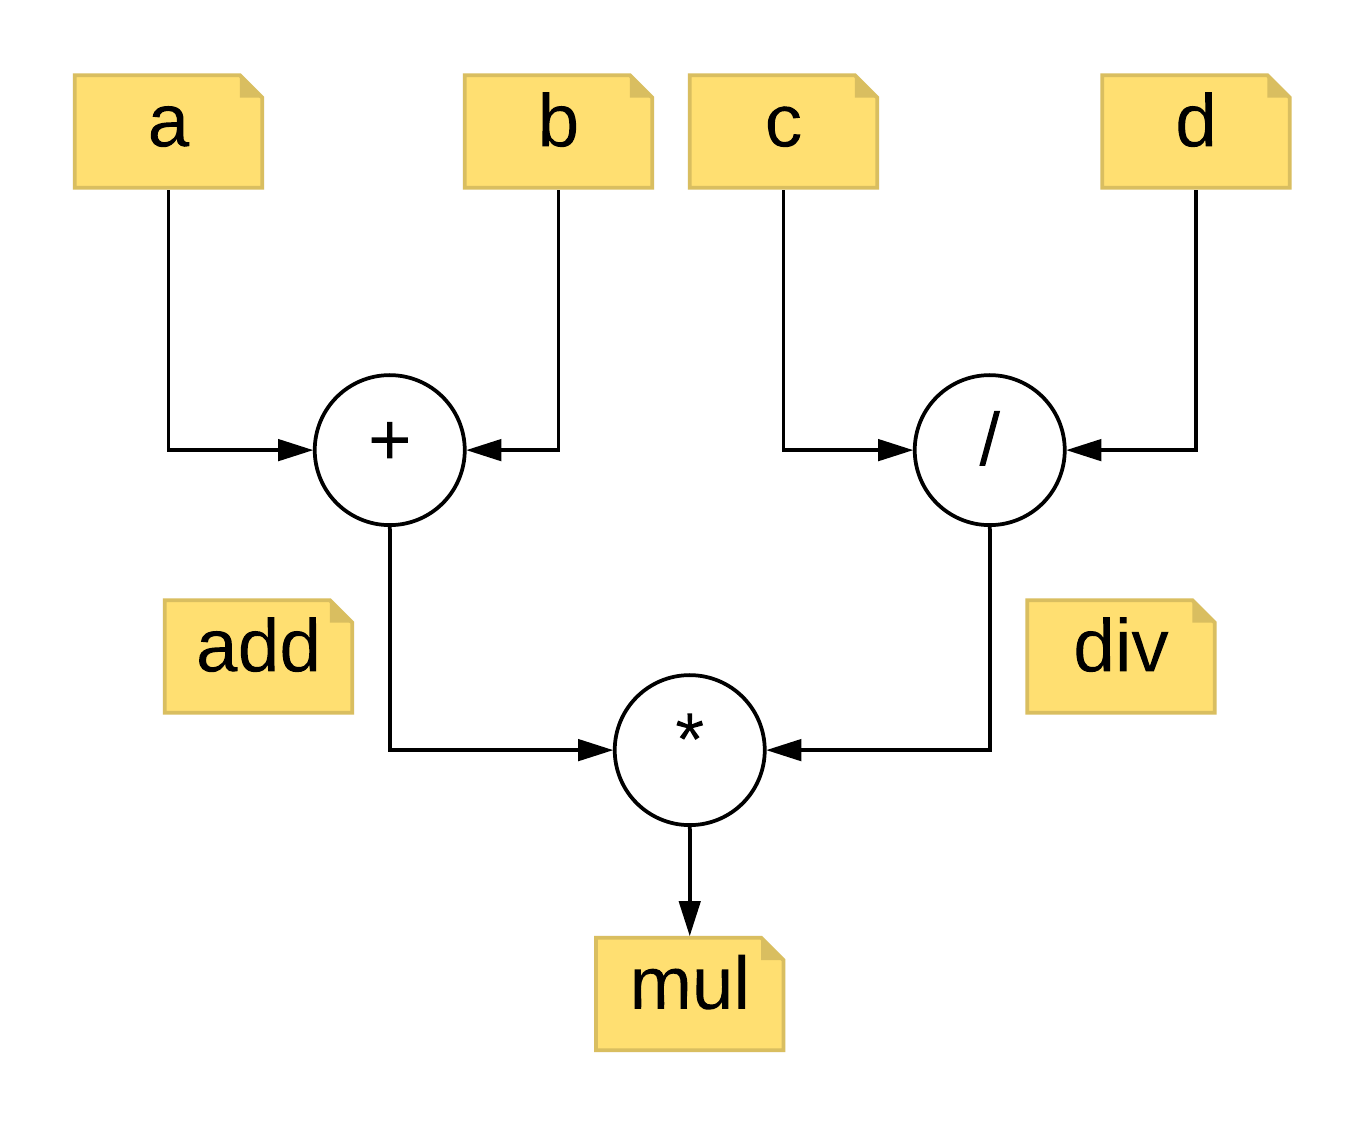
\includegraphics[width=.75\linewidth]{Figures/Circuit.png}
    \caption{Example Arithmetic Circuit}
    \label{fig:circuit}
\end{figure}

\FloatBarrier
\subsection{R1CS Form}
The next step of generating a proof is making sure that all constraints in the circuit are satisfied (eg. that multiplication gates actually perform multiplication). This is achieved by conversion of the circuit into R1CS form (Rank 1 Constraint System). Circuits consist of gates and wires. Gates perform operations and wires carry values. R1CS makes sure that values satisfy constraints set by the gates.\\
\\
R1CS for a gate consists of 4 vectors: \textbf{S}, \textbf{A}, \textbf{B}, and \textbf{C}. Vector \textbf{S} represents the assignments of values to all wires in a circuit, and a value 1. It is also called a witness. Vectors \textbf{A}, \textbf{B}, and \textbf{C} represent the constraints. They are filled based on the operation the gate performs, in such way that the constraint in Equation \ref{eq:r1cs} is met.

\begin{equation}
    \label{eq:r1cs}
    \textbf{A}_i \cdot \textbf{S} \times \textbf{B}_i \cdot \textbf{S} - \textbf{C}_i \cdot \textbf{S} = 0
\end{equation}

\noindent If we take a look at the multiplication gate in Figure \ref{fig:circuit}, we can construct the following R1CS representation:

\begin{figure}[h]
    \centering
    \includegraphics[width=.5\linewidth]{Figures/{"MUL R1CS"}.png}
    \caption{Multiplication Gate R1CS}
    \label{fig:mulr1cs}
\end{figure}

\FloatBarrier

\noindent The first thing that we notice in Figure \ref{fig:mulr1cs} is that there is no wire marked \textbf{add}. Addition (and subtraction) can be folded into multiplication and division gates, so we can reduce the number of wires. Wire \textbf{add} has been replaced by inputs of the addition gate \textbf{a} and \textbf{b}. These values have been assigned value \textbf{1} in vector \textbf{A} -- they appear once in the first argument of multiplication. Wire \textbf{div} appears once in right argument (vector \textbf{B}), while wire \textbf{mul} is marked in the output (vector \textbf{C}). Calculating the constraint shows that Equation \ref{eq:r1cs} is satisfied.\\\\

\begin{figure}[h]
    \centering
    \includegraphics[width=.5\linewidth]{Figures/{"DIV R1CS"}.png}
    \caption{Division Gate R1CS}
    \label{fig:divr1cs}
\end{figure}

\noindent Figure \ref{fig:divr1cs} shows R1CS for the division gate in Figure \ref{fig:circuit}. R1CS for this gate actually guarantees that $\textbf{div} \cdot \textbf{d} = \textbf{c}$, which is equivalent to $\textbf{c} / \textbf{d} = \textbf{div}$. Vector \textbf{A} contains the coefficient for \textbf{div}, while vector \textbf{B} contains the value connected to the divisor \textbf{d}. The dividend \textbf{c} has been assigned a value of 1 in vector \textbf{C}. Equation \ref{eq:r1cs} is also satisfied in this case.

\FloatBarrier

\subsection{Quadratic Arithmetic Program}
Quadratic Arithmetic Program enables us to represent R1CS constraints for all gates at once. First, we enumerate all gates, and construct three polynomials (A(x), B(x), and C(x)) for every wire in the circuit. Polynomial for the j-th variable $A_j(x)$ is formed by interpolating it through the points with coordinates $(i, \textbf{A}_j^i)$. Here, $i$ represents the gate index and $\textbf{A}_j$ represents the entry assigned to $j^{th}$ wire. 
%, where GateIndex is the index assigned to gate when they were enumerated, $A_{GateIndex}$ is the corresponding A vector, and $A_{GateIndex} [i]$ is the value of the i-th constant in the vector
Polynomials can be interpolated using well-known algorithm such as Langrangian interpolation. We can recover R1CS vectors by calculating values of the polynomials at the gate's index (Example \ref{ex:recover}).

\begin{exmp}
\label{ex:recover}
If we want to recover the $2^{nd}$ gate's value assigned to $4^{th}$ wire in vector \textbf{B} -- $\textbf{B}_4^2$, we can do it by computing $B_4(2)$.
\end{exmp}

\noindent Then, we form a new polynomial A(x) by arranging all $A_j$ vectors in a new vector based on the index j, and taking a scalar product with \textbf{S}. We form polynomials B(x) and C(x) the same way. The number of wires (variables) in a circuit is denoted by \textit{w}.

\begin{equation}
    \label{eq:polydef}
A(x) = \sum_{j = 1}^{w} \textbf{S}^j \cdot A_j(x)
\end{equation}

\noindent Considering that polynomials A(x), B(x) and C(x) are sums of interpolated polynomials multiplied by the corresponding element in \textbf{S}, we can evaluate them at different indices and derive Theorem \ref{theorem:zero}. The total number of gates in a circuit is denoted by \textit{g}.



\begin{theorem}
    \label{theorem:zero}
    $$\forall t:\: [t \in \{1,\,2,\,3, \dots g\} \implies A(t) \cdot B(t) - C(t) = 0]$$
\end{theorem}

\begin{proof}
    We know that Equation \ref{eq:r1cs} holds for every gate:

    $$\forall t:\: [t \in \{1,\,2,\,3, \dots g\} \implies \textbf{A}_t \cdot \textbf{S} \times \textbf{B}_t \cdot \textbf{S} - \textbf{C}_t \cdot \textbf{S} = 0]$$

    \noindent We can expand every scalar product into a sum over all \textit{n} wires:

    $$\forall t:\: [t \in \{1,\,2,\,3, \dots g\} \implies (\sum_{j = 1}^{n} \textbf{A}_t^j \cdot \textbf{S}^j) \times (\sum_{j = 1}^{n} \textbf{B}_t^j \cdot \textbf{S}^j) - (\sum_{j = 1}^{n} \textbf{C}_t^j \cdot \textbf{S}^j) = 0]$$

    \noindent By definition, a polynomial interpolated from some points has the same values when evaluated at those points, so we can substitute them:

    $$\forall t:\: [t \in \{1,\,2,\,3, \dots g\} \implies (\sum_{j = 1}^{n} A_j(t) \cdot \textbf{S}^j) \times (\sum_{j = 1}^{n} B_j(t) \cdot \textbf{S}^j) - (\sum_{j = 1}^{n} C_j(t) \cdot \textbf{S}^j) = 0]$$

    \noindent We can use the definition of polynomials A(x), B(x), and C(x) (Equation \ref{eq:polydef}) to conclude that Theorem \ref{theorem:zero} is true.

    $$\forall t:\: [t \in \{1,\,2,\,3, \dots g\} \implies A(t) \cdot B(t) - C(t) = 0]$$

\end{proof}

\begin{theorem}
    \label{theorem:div}
    Theorem \ref{theorem:zero} implies that the polynomial $A(x) \cdot B(x) - C(x)$ is divisible by the polynomial $T(x) = (x-1)(x-2)\dots(x-g)$, or more formally:

    $$ A(x) \cdot B(x) - C(x) = T(x) \cdot H(x) $$

\end{theorem}

\begin{proof}
    From \ref{theorem:zero} we know that 1, 2, 3\dots g are roots of the polynomial $A(x) \cdot B(x) - C(x)$. We can now use the factor theorem. The first $g$ factors correspond to known roots of the polynomial, while $H(x)$ represents the coefficient:

    $$ A(x) \cdot B(x) - C(x) = (x-1)(x-2)\dots(x-g) \cdot H(x) $$

    \noindent The first part is actually just $T(x)$ so we subsitute it, finishing the proof.

    $$ A(x) \cdot B(x) - C(x) = T(x) \cdot H(x) $$

\end{proof}

\subsection{Pinocchio Protocol}

This section presumes basic (operational) knowledge of elliptic curves and pairings. In his articles Buterin provides a decent, albeit non-technical, introduction to both elliptic curves and pairings \cite{buterin1, buterin2, buterin3}. For a short black-box treatment of different cryptographic pairings, consult \cite{galbraith2008pairings}. Readers looking for a more textbook introduction to pairings, can read \cite{costello2012pairings}.\\
\\
The simplest way to verify that all checks that the circuit, or QAP, performs are satisfied, would be to reveal all values. However, that would leak sensitive information such as private keys, available funds, transferred ZEC, etc. Providing just a polynomial divisible by T(x) would be meaningless, because it could have been forged. The primitive we need should provide us with a way to check that the polynomial was constructed in a specific way, while letting us verify that it is indeed divisible by T(x). Pinocchio protocol \cite{parno2013pinocchio} uses  pairings (bilinear maps) to achieve that goal.\\
\\
In this section, we use a type III pairing: $e: \mathbb{G}_1 \times \mathbb{G}_2 \to \mathbb{G}_T$. A pairing is denoted by a two-argument function $e(P_{G_1}, P_{G_2})$. $G_1, G_2$ and $G_T$ represent generators of groups $\mathbb{G}_1$, $\mathbb{G}_2$ and $\mathbb{G}_T$, respectively. All group operations are represented in the additive notation to stress that we are working with elliptic curve points (+ for the operations in $\mathbb{G}_1$ and $\mathbb{G}_2$, $\oplus$ for $\mathbb{G}_T$ , and $[n]P$ for scalar multiplication for all groups).\\
\\
\begin{exmp}
    \label{pairingexample}
    Pairings can be used to check whether two pairs of elliptic curve points (A and B, C and D) have the same quotients:

    $$ B / A \stackrel{?}{=} D / C $$
    This is verified by computing two pairings:
    $$ e(A, D) \stackrel{?}{=} e(B, C) $$
    In case of $A = [k]B; C = [k]D$ we have:
    $$ e([k]B, D) \stackrel{?}{=} e(B, [k]D)$$
    We use property of the pairing to move the constant outside the pairings:
    $$ [k]e(B, D) = [k]e(B, D) $$
    If the pairs have the same quotients, both pairings will be equal. $\square$
\end{exmp}

\noindent As we mentioned in Section \ref{section:zkproofs} that non-interactive proofs must rely either on a common reference string (CRS), or some shared randomness equivalent to CRS (eg. random oracle). Unless the CRS is created correctly, and all private data is deleted after its creation, it is vulnerable to backdooring. Any person that knows that information can create fake proofs. This is where the term trusted setup originates. In order for proofs to be secure, the party creating it must strictly follow the procedure. As we will see in Section \ref{section:rust}, Zcash has used many different techniques to reduce the risk as much as possible.\\
\\
The most important piece of information that needs to be destroyed after we create CRS, is the coordinate $t$ at which polynomials A(x), B(x) and C(x) will be evaluated. There is also a paradox here to resolve: Although $t$ needs to be secret, we must allow the prover to calculate the values of polynomials at $t$. This is achieved by multiplying the powers of $t$ by $G_1$, and adding them to the CRS. These powers will be used later to compute $[H(t)]G_1$. We presume that the discrete logarithm problem (DL) is hard, so the adversary cannot extract $t$ from the powers.\\
\\
To obtain $A(t), B(t), C(t)$ we need to compute $A_j(t), B_j(t), C_j(t)$ for all gates in the circuit. By also adding these values multiplied by secret coefficients $k_a, k_b$ and $k_c$ to the CRS, and using the idea from Example \ref{pairingexample}, we are able to prevent the prover from using arbitrary polynomials. Multiplication by the elliptic curve generator enables us to also perform the needed pairing checks. Values $\rho_A, \rho_B, \beta, \gamma$ are also considered secret, and are used to aid subsequent pairing checks. Accordingly, we add the following values to the trusted setup:

$$\forall j \in \{1, 2, 3, \ldots g\} : [\rho_A A_j(t)]G_1, [k_A \rho_A A_j(t)]G_1 $$
$$\forall j \in \{1, 2, 3, \ldots g\} : [\rho_B B_j(t)]G_2, [k_B \rho_B B_j(t)]G_1 $$ 
$$\forall j \in \{1, 2, 3, \ldots g\} : [\rho_A \rho_B C_j(t)]G_1, [k_C \rho_A \rho_B C_j(t)]G_1 $$ 

\noindent The prover then needs to provide the following points to prove that they computed polynomials $A(x), B(x), C(x)$ correctly:

$$\pi_A = [\rho_A A(t)]G_1, \pi_A' = [k_A \rho_A A(t)]G_1$$
$$\pi_B = [\rho_B B(t)]G_2, \pi_B' = [k_B \rho_B B(t)]G_1$$
$$\pi_C = [\rho_A \rho_B C(t)]G_1, \pi_C' = [k_C \rho_A \rho_B C(t)]G_1$$

\noindent The check is performed by computing:

$$ e(\pi_A, [k_a]G_2) \stackrel{?}{=} e(\pi_A', G_2) $$
$$ e([k_b]G_1, \pi_B) \stackrel{?}{=} e(\pi_B', G_2) $$
$$ e(\pi_C, [k_c]G_2) \stackrel{?}{=} e(\pi_C', G_2) $$

\noindent Considering that polynomials $A(x), B(x), C(x)$ are linear combinations of polynomials $A_j(x), B_j(x), C_j(x)$, respectively, required points can be computed from the points in the trusted setup and the witness \textbf{S} (\textbf{S} represents the coefficients of linear combination). Notice that the verifier needs $G_1$, $G_2$, $[k_a]G_2$, $[k_b]G_1$, $[k_c]G_2$ to perform the check, so we also need to add them to the CRS. No one can retrieve $k_a$, $k_b$, nor $k_c$ if DL is hard.\\
\\
The prover must also convince the verifier that they have used the same coefficients for all polynomials. This is achieved by extending the trusted setup with the following points:

$$\forall j \in \{1, 2, 3, \ldots, g\} : [\beta(\rho_A A_j(t) + \rho_B B_j(t) + \rho_A \rho_B C_j(t))]G_1 $$

\noindent The prover then provides the point:

$$ \pi_{K} = [\beta(\rho_A A(t) + \rho_B B(t) + \rho_A \rho_B C(t))]G_1 $$

\noindent Pairing check is performed by the verifier:

$$ e(\pi_K, [\gamma]G_2) \stackrel{?}{=} e(\pi_A + \pi_C, [\gamma\beta]G_2) \oplus e([\gamma\beta]G_1, \pi_B) $$

\noindent Finally, they need to prove that the polynomial $A(x) \cdot B(x) - C(x)$ is really divisible by $T(x)$. This is achieved by using the polynomial $H(x)$ to show that multiplying it by $T(x)$ gives us $A(x) \cdot B(x) - C(x)$. If the prover provides $\pi_H = [H(t)]G_1$, we can do this using pairings:

$$ e(\pi_a, \pi_b) \stackrel{?}{=} e(\pi_c, G_2) \oplus e(P_H, [\rho_A \rho_B T(t)]G_2) $$

\noindent We will now discuss the simplifications made to the proof. The proof explained works for proofs without any input wires. Adding inputs to the circuit is straightforward. It involves introducing several terms to the CRS and adding them to $\pi_A$ during the linearity and divisibility checks. The reader can check the full version of Pinocchio zk-SNARKs in \cite{parno2013pinocchio}, or just the review at the end of \cite{ben2014succinct}.\\
\\
There is another important place where we deviate from Buterin's articles: We use asymmetric pairing, instead of A symmetric pairing. Asymmetric pairings are more efficient and make Groth's results in the section \ref{grothexpl} easier to understand.\\
\\
The final remark has to do with the choice of groups $\mathbb{G}_1$ and $\mathbb{G}_2$ for the points provided by the prover. All points beside $\pi_B$ are elements of $\mathbb{G}_1$. Elements of $\mathbb{G}_1$ are smaller than the elements of $\mathbb{G}_2$. Pinocchio protocol takes advantage of this to reduce the size of the proof by assign as many points as possible to $\mathbb{G}_1$. $\pi_B$ is the only point that has to be in $\mathbb{G}_2$ due to the pairing check where we calculate $e(\pi_A, \pi_B)$. This brings us to the proof consisting of 7 $\mathbb{G}_1$ and 1 $\mathbb{G}_2$ element.

\section{Sapling Update}

\subsection{Introduction}
Zcash is undergoing continuous development. The most substantial update to date is called Sapling \cite{zcashsapling}. Its goal was to overhaul the cryptography of Zcash. The major changes are a new curve, new commitment scheme, a new proving system, as well as writing these components in Rust. The changes are meant to address the slow speed of shielded transactions, and lead to their wider adoption.

\subsection{New Curve: BLS12-381}

The old curve BN254 saw its conservative security level estimate reduced to 110 bits after a new variant of the number sieve algorithm was presented \cite{zcashbls12381, cryptoeprint:2015:1027}. Increasing the security parameters for this curve would reduce the performance of FFT (for polynomial division) and multiexponentiation steps of proof generation. A new curve was selected - BLS12-381. The embedding degrees of this curve is 12. Other parameters of this curve are its group order $r \approx 2^{255}$ and the base field characteristic $q \approx 2^{381}$.

\subsection{New Commitment Scheme: Pedersen Commitments and JubJub}

Zcash zk-SNARK circuit needs to compute and verify commitments to notes. SHA256 compression function was used as the commitment scheme. Unfortunately, this also bloated the circuit quite a bit. The move to BLS12-381 did not only increase the security level to 128 bits, but also introduce a highly efficient commitment scheme: Pedersen commitments over a custom Edwards curve Ed255-JubJub \cite{zcashjubjub}. The field underlaying JubJub can fit in the scalar field of BLS12-381 and be calculated in the circuit quite efficiently. This change alone reduced shielded transaction generation time by 75\% \cite{zcashreducing}.

\subsection{New Proving System}
\label{grothexpl}

While Pinocchio is fullfulls all requirements for Zcash, its biggest problem is the proof size. Instead of using 7 $\mathbb{G}_1$ elements, and one $\mathbb{G}_2$ element, Jens Groth \cite{groth2016size} improved upon the previous work to use only 2 $\mathbb{G}_1$ elements and a $\mathbb{G}_2$ element. He also proved that at least one element needs to be in each group for linear circuit checks to be secure.\\
\\
The new system has the prover provide:

$$ \pi_A = [\underbrace{\alpha + A(t) + r\delta}_\text{X}]G_1 $$
$$ \pi_B = [\underbrace{\beta + B(t) + s\delta}_\text{Y}]G_2 $$
$$ \pi_C = [\frac{\beta A(t) + \alpha B(t) + C(t) + H(t)T(t)}{\delta} + Xs + Yr - rs\delta]G_1 $$

\noindent The verifier needs to check:

$$ e(\pi_A, \pi_B) \stackrel{?}{=} e(\alpha G_1, \beta G_2) \oplus e(\pi_C, \delta G_2) $$

\noindent Groth's zk-SNARK has been simplified here and doesn't include inputs to the circuit. Constants $\alpha, \beta, \delta, r, s, t$ are random secrets generated during the generation of CRS. Polynomials A(x), B(x), C(x), H(x), and T(x) are defined in the same way as in Pinocchio \cite{parno2013pinocchio} protocol.

\subsection{Rust Implementation}
\label{section:rust}
Rust \cite{rustlang} was imagined as a memory-safe and thread-safe low-level programming language. Switching to a new curve required a rewrite of the cryptographic code. This was done in Rust to improve the security of Zcash \cite{zcashbellman}. Furthermore, a new trusted setup was required to define the CRS for Groth's proving system. The program for the ceremony was also written in Rust and used secure multiparty computation to guarantee honesty. 87 people contributed in the first (circuit-agnostic) phase, and over 90 took part in the second phase \cite{zcashparamgen}.
% Chapter Template

\chapter{OpenCL} % Main chapter title

\label{Chapter4} % Change X to a consecutive number; for referencing this chapter elsewhere, use \ref{ChapterX}

%----------------------------------------------------------------------------------------
%	SECTION 1
%----------------------------------------------------------------------------------------

\section{History and Introduction}

With the predictions of the Moore's Law \cite{moore1965cramming} coming to an end for single-core processors, new programming and hardware paradigm was needed to continue the exponential growth. Increasing the frequency of the chip to improve performance would have resulted in overheating (Power Wall). Furthermore, manufacturers continued to reduce the size of a transistor, giving them more computing elements to work with. The answer was reducing the frequency, but using extra transistors to exploit various levels of parallelism present in programs.\\
\\
CPU manufacturers (Intel, AMD) needed to maintain the performance of single-threaded applications intact while expoliting thread-level parallelism. They opted to have a small number of independent cores in their processors (eg. Intel Dual Core). This was complemented by the invention of hyperthreading \cite{marr2002hyper} which enabled a single core to execute multiple instruction streams simultaneously.\\
\\
GPU computing took a different route \cite{mcclanahan2010history}. GPU loads were already massively parallel - small programs were applied to every pixel on the screen. This resulted in GPUs having hundreds of small processor, performing the same computation on different data (SIMD - Single Instruction Multiple Data). Unfortunately, even though their computing power continued to grow, graphics cards were limited to performing only computations limited to image processing. This changed with OpenGL 2.0 standard released in 2004 \cite{segal2004opengl}. Even though OpenGL is a graphics API, it enabled users to write general-purpose code using GLSL \cite{kessenich2004opengl}. Soon, NVIDIA published their own general-purpose GPU solution - CUDA \cite{nvidia2007nvidia}.\\
\\
With so much different parallel hardware on the market, interoperability was hard to achieve. Someone having an ATI GPU could not run CUDA programs, so they were forced to buy a new graphics card, or port their software to OpenGL 2.0 which was meant to be used for graphics. In 2009. Apple published OpenCL to provide heterogenous computing support on as many platforms as possible. Only OpenCL architecture is standardized, so the actual, underlying implementation (organization) is left to hardware vendors. This means that OpenCL programs can take full advantage of available hardware - GPUs will execute them in SIMD fashion, FPGA compilers will create only needed SIMD hardware, while multi-core CPUs will run the program in multiple threads. Today, OpenCL is supported on multi-core CPUs, integrated CPU graphics, GPUs, FPGAs, and by almost all major hardware manufacturers (Intel, AMD, NVIDIA, ARM...).


%----------------------------------------------------------------------------------------
%	SECTION 2
%----------------------------------------------------------------------------------------

\section{OpenCL Architecture}

Information in this section is based on \cite{gaster2012heterogeneous}.

\subsection{Host and Kernel}

OpenCL program consists of two parts: host program and a guest program (kernel) (Figure \ref{fig:openclplatform} \cite{munshi2009opencl}). Host program is written in a language which has OpenCL bindings available (C, C++, Python, Rust\dots), while the kernel is written in OpenCL C or OpenCL C++ (OpenCL 2.1+). Host application interfaces with the operating system to find out which OpenCL devices are available, compiles kernels, queues them for execution and reads back the result. Kernel receives parameters from the host application, performs (usually parallel) operations and returns the result.

\begin{figure}[h]
    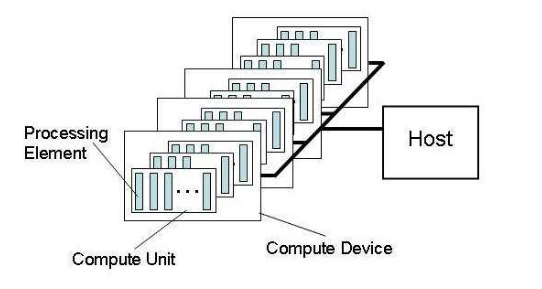
\includegraphics[width=\linewidth]{Figures/platform.png}
    \caption{OpenCL Platform Model}
    \label{fig:openclplatform}
\end{figure}

To help parallelization, many instances of kernel are run, each having a different ID. Based on its ID, kernel decided which data to fetch, and which operations to execute. Several kernel instances can form a group, which can be used to partially synchronize execution of more complex kernel. Host program determines the total number of kernel instances, as well as the size of a group.

\subsection{Memory Hierarchy}
OpenCL was heavily influenced by CUDA, which is evident in the organization of memory (Figure \ref{fig:openclmemory} \cite{munshi2009opencl}). While CPUs usually automatically handle latency hiding by caching frequent accesses, there are no guarantees that OpenCL devices have cache onboard. The developer must choose where data resides.

\begin{figure}[h]
    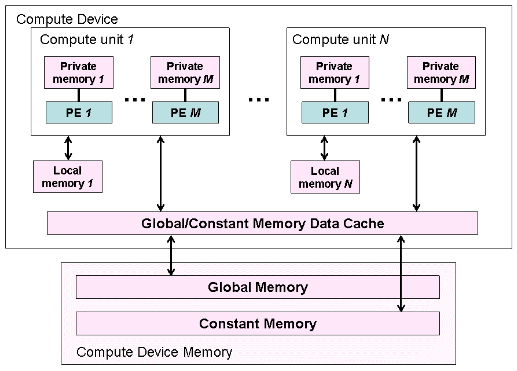
\includegraphics[width=\linewidth]{Figures/memory.png}
    \caption{OpenCL Memory Model}
    \label{fig:openclmemory}
\end{figure}

There are three levels of memory, each smaller, faster and accessible by a smaller number of elements than the last. Devices differ in the amount of memory available at each level. If the kernel uses more memory than available, accesses will spill to a lower memory level, slowing down memory accesses.
\begin{itemize}
    \item \b{Global memory} (\texttt{\_\_global}) is accessible by every kernel instance, as well as by a host application (using OpenCL calls). This is where host usually writes starting data, and where kernel outputs results. It has the longest latency, but also the highest capacity. \b{Constant memory} (\texttt{\_\_constant}) is a special part of global memory where read-only data can be stored.
    \item \b{Local memory} (\texttt{\_\_local}) is accessible by the elements in the same group.
    \item \b{Private memory} (no keyword) is accessible only by its owner. It is the fastest, but also the smallest memory.
\end{itemize}

\subsection{Latency Hiding}

While OpenCL is indeed platform-agnostic, organizational details of GPUs affect the performance of OpenCL code running on them. GPUs consist of thousands of compute units split into groups which execute same instructions in parallel. When a unit issues a data request, the thread blocks until it is served. If there is free space in the register file, the scheduler will start the execution of the next segment. This can happen as many times as needed, as long as there are free registers. If a kernel is well optimized, the GPU will almost never be idle.\\
\\
This leads to two opposite concepts to keep in mind when writing OpenCL kernels for GPUs. Caching frequently used data in local and private memory (without overflowing to lower hierarchies) reduces latency for subsequent accesses. Unfortunately, this also reduces the number of threads whose state we can keep simultaneously. Balancing these two forces leads to the fastest execution of a kernel.\\
% The following sentence should be moved to the chapter about implementation
%Today, OpenCL compilers often use LLVM and perform many different optimization runs on kernel code. Hand-optimizing register usage to an extent that makes code unreadable, as well as performing trivial changes in the code, should be avoided because compilers will usually generate the same code. Developers should focus on things compilers can't and shouldn't optimize - algorithmic improvements and use of memory hierarchy.
 
\chapter{Implementation Details} % Main chapter title

\label{Chapter5} % Change X to a consecutive number; for referencing this chapter elsewhere, use \ref{ChapterX}

%----------------------------------------------------------------------------------------
%	SECTION 1
%----------------------------------------------------------------------------------------

\section{Implementation of Elliptic Curve Operations}


Rust implementation of BLS12-381 from the pairing crate \cite{githubpairing} used by zCash was ported to OpenCL C. This step was straight-forward and made easier by the fixed size of primitive data types in both Rust and OpenCL C. Constants were used wherever it was possible, to aid compiler optimization. Almost all functions were inlined to remove the function call overhead and open new opportunities for optimization. Due to the difficulty in debugging on GPUs and cryptographic code, almost every function is unit tested and compared to the Rust implementation.\\
\\
The host code is written in Rust to interface with the librustzcash Rust library \cite{githublibrustzcash}, and uses ocl crate \cite{githubocl}. The higher level interface is used for testing on Intel, NVIDIA and AMD GPUs. However, cross-compilation for Android some tests had to be implemented using the low-level API.\\
\\
Finite fields $\mathbb{F}_r$ (255-bit modulus) and $\mathbb{F}_q$ (381-bit modulus) have been ported to OpenCL, as well as an elliptic curve BLS12-381 group $\mathbb{G}_1$ over $\mathbb{F}_q$.

\section{Multiexponentiation Algorithms}

\subsection{Pippenger's Multiexponentiation Algorithm}
The most time-consuming part of proof generation is the multiplication of the elliptic curve points by the coefficients of the witness to create $\pi_A$, $\pi_B$ and $\pi_C$. In the multiplicative notation, this multiplication becomes exponentiation, so the algorithms solving this problem can also be called exponentiation algorithms.\\
\\
The actual problem we are trying to solve is:\\
\\
Given $x_1$, $x_2$,\dots, $x_n$ $\in \mathbb{G}$ and $y_1$, $y_2$,\dots, $y_n \in \mathbb{Z}$, compute $x_1^{y_1} x_2^{y_2} \dots x_n^{y_n}$.\\
\\
While square-and-multiply (Figure \ref{fig:sam}) and the sliding window method (Figure \ref{fig:wsam}) are asymptotically optimal for a single exponentiation, it is possible to compute the multiexponentiation faster by grouping terms, and exponentiating them together.\\
\\
\textbf{Example:} $2^3 5^3$ can be computed as $(2 \cdot 5)^3$.\\
\\
Pippenger's multiexponentiation algorithm \cite{pippenger1976evaluation} can be used to calculate the required product. The algorithm can be used to calculate several multiproducts at once ($x_1^{y_1} x_2^{y_2} \dots x_n^{y_n}$, $x_1^{z_1} x_2^{z_2} \dots x_n^{z_n}$, $x_1^{p_1} x_2^{p_2} \dots x_n^{p_n}$) and Pippenger has proven that the algorithm is asymptotically optimal. However, for zk-SNARKs we require only one multiexponentiation, so the actual implementation is slightly simpler. For background on Pippenger's algorithm consult \cite{henry2010pippenger}. Another paper on Pippenger, as well as some alternatives (such as Yao's \cite{yao1976evaluation} and Brauer \cite{brauer1939addition}) is \cite{bernstein2002pippenger3s}. For discussion and computational comparison of several methods (including Bos-Coster algorithm \cite{bos1989addition}) check \cite{bergeron1994efficient}. In the rest of the section, we will discuss theversion of the Pippenger from bellman Rust crate (Figure \ref{fig:multiexp}).
\begin{algorithm}[h]
\caption{Simplified Pippenger}\label{fig:multiexp}
\begin{algorithmic}[1]
\Function{MultiexpInner}{\textit{Bases}[1 \dots n], \textit{Exponents}[1 \dots n], \textit{Shift}, \textit{Width}}

    \If{$Shift + Width < EXP\_BITS$}
        \State $Higher \gets \textbf{new thread}$ \Call{MultiexpInner}{\textit{Bases}, \textit{Exponents}, \textit{Shift}+\textit{Width}, \textit{Width}}
    \EndIf
    \State $Buckets \gets \textbf{new} \; Base[1\dots2^{Width}-1]$
    \State $Mask \gets 2^{Width}-1$
    \For{$i \gets 1 \dots n$}
        \State $ExpPart \gets (Exponents[i] \gg Shift) \; \&  \;Mask$
        \If{$ExpPart \neq 0$}
            \State $Buckets[ExpPart] \gets Buckets[ExpPart] \cdot Bases[i]$
        \EndIf
    \EndFor
    
    \State $PartialSum \gets 0$
    \State $Sum \gets 0$
    
    \For{$i \gets 2^{Width}-1 \dots 1$}
        \State $PartialSum \gets PartialSum \cdot Buckets[i]$
        \State $Sum \gets Sum \cdot PartialSum$
    \EndFor
    
    \If{$Shift + Width < EXP\_BITS$}
        \State \textbf{wait} $Higher$
        \For{$i \gets Width \dots 1$}
            \State $Higher \gets Higher \cdot Higher$
        \EndFor
        \State $Sum \gets Sum \cdot Higher$ 
    \EndIf
    
    \State \textbf{return} $Sum$
\EndFunction
\\
\Function{Multiexp}{\textit{Bases}[1 \dots n], \textit{Exponents}[1 \dots n]}
    \If{n < 32}
        \State $Width \gets 3$
    \Else
        \State $Width \gets ln(n)$
    \EndIf

    \State \textbf{return} \Call{MultiexpInner}{$Bases$, $Exponents$, $0$, $Width$}
    
\EndFunction
\end{algorithmic}
\end{algorithm}

The algorithm segments the exponents in chunks of several bits. Every thread then iterates through the assigned bits, and based on them, adds bases to corresponding buckets. Buckets are then added in an efficient way:

$$ a + 2b + 3c = c + (c + b) + (c + b + a) $$

Afterward, we wait for higher threads to finish, and combine results.\\
\\
As we can see this algorithm is quite parallelizable. We just need to change the width of the bit chunk to distribute work over more threads. Another possibility is to split the bases and exponents and do the calculation separately. However, we notice some limitations as well. There is sequential work that needs to be done when we are combining results. We cannot split the work on more processors than there are bits in the exponent, without splitting the bases to different processors. This would add another sequential step in the end to combine all intermediate results.
\\
\subsection{Implemented Algorithms}

% \subsubsection{Global Reduction}
% Global reduction kernel performs one step of reduction. It loads two elliptic curve points in projective coordinates, adds them, and writes them back to the memory. This kernel is called multiple times, with half the length every time, until we add all points together.
% \subsubsection{Local Reduction}
% Local reduction kernel tries to take advantage of faster local memory available on a GPU. It loads a group of points to local memory, and reduces them until only one point is left. Compared to the global reduction kernel, it uses more local memory, and as reduction progresses many computing units don't do any work. However, it needs to be called less times, and the number of loads from the global memory is significantly smaller.

\subsubsection{Square and Multiply (Binary Method)}

\begin{algorithm}[h]
    \caption{Square and Multiply Algortihm }\label{fig:sam}
    \begin{algorithmic}[1]
    \Function{SAM}{\textit{Base}, \textit{Exponent}}
    
        \State $Result \gets 1$
        \For{$i \gets Width \dots 1$}
            \State $Result \gets Result^2$
            \If{$Exponent[i] = 1$}
                \State $Result \gets Result \cdot Base$
            \EndIf
        \EndFor
        \State \textbf{return} $Result$
    \EndFunction
    \\
    \Function{Multiexp}{\textit{Bases}[1 \dots n], \textit{Exponents}[1 \dots n]}
        \State $Result \gets 1$
        \For{$i \gets 1 \dots n$}
            \State $Result \gets Result \cdot $\Call{SAM}{$Bases[i]$, $Exponents[i]$}
        \EndFor
    
        \State \textbf{return} $Result$
        
    \EndFunction
    \end{algorithmic}
\end{algorithm}
Square-and-multiply\footnote{Double-and-add in additive groups} \cite{knuth2014art} (Figure \ref{fig:sam}) multiexponentiation kernel implements multiexponentiation in a simple way. Every elliptic curve point and exponent is loaded, exponentiated separately using the binary method, and written back to memory. Reduction algorithm is then called to produce the final result.
\subsubsection{Sliding Window Method}
\begin{algorithm}[h]
    \caption{Sliding Window Method}\label{fig:wsam}
    \begin{algorithmic}[1]
    \Function{SWM}{\textit{Base}, \textit{Exponent}}
        \State $PowerTable[1 \dots Chunk] \gets \textbf{new} Base[1 \dots Chunk]$
        \State $CurrentPower \gets 1$
        \\
        \For{$i \gets 1 \dots Chunk$}
            \State $CurrentPower \gets CurrentPower \cdot Base$
            \State $PowerTable[i] \ gets CurrentPower$
        \EndFor
        \\
        \State $Result \gets 1$
        \For{$i \gets Width/Chunk \dots 1$}
            \State $Bits \gets $ \textit{Get }$i^{th}$ \textit{ Chunk From Exponent}
            \For{$j \gets 1 \dots Chunk$}
                \State $Result \gets Result^2$
            \EndFor
            \\
            \If{$Bits \neq 0$}
                \State $Result \gets Result \cdot PowerTable[Bits]$
            \EndIf
        \EndFor
        \\
        \State \textbf{return} $Result$
    \EndFunction
    \\
    \Function{Multiexp}{\textit{Bases}[1 \dots n], \textit{Exponents}[1 \dots n]}
        \State $Result \gets 1$
        \For{$i \gets 1 \dots n$}
            \State $Result \gets Result \cdot $\Call{SWM}{$Bases[i]$, $Exponents[i]$}
        \EndFor
    
        \State \textbf{return} $Result$
        
    \EndFunction
    \end{algorithmic}
\end{algorithm}
Sliding window method \cite{knuth2014art} \ref{fig:wsam} is a generalization of square-and-multiply. It also works with every point and exponent separately, but it processes the exponent 4 bits at a time. First, a lookup table is generated for the powers of the current base (powers 2-15). For every chunk of the exponent read, it performs the needed amount of squarings and adds the corresponding power. This method uses more memory than ordinary square-and-multiply, but the number of operations is lower.
\subsubsection{Four-bit Pippenger's Algorithm}
This kernel is the closest to the Rust implementation of Pippenger's algorithm (Figure \ref{fig:multiexp}). Points are divided in chunks to take advantage of thousands of processors on the GPU. Every thread then iterates through the points in the chunk and reads the four-bit window in the exponent based on the thread index. Point is then added to the corresponding bucket. In the end, we add the buckets and write the result to shared local memory. Then we combine results from all threads working on the same chunk. This is done by a variation of a reduction algorithm working only on local memory. The chunk value is then written to global memory, and a reduction algorithm is called to combine all chunks together.
\subsubsection{One-bit Pippenger's Algorithm}
In this implementation of Pippenger's algorithm (Figure \ref{fig:multiexp}), points are divided into multiple chunks. Kernel threads are grouped in blocks of 256, and every thread is assigned to a bit in the exponent. Every thread iterates through the points in its chunk and adds all points where the tracked bit is one. When they are finished, threads write the results to the global memory. These sums are then reduced based on the bit in the exponent which was assigned to them. Finally, these 256 values are added together using the efficient addition algorithm from the previous section.
\subsubsection{Four-bit Pippenger's Algorithm with Separate Reduction}
Four-bit Pippenger's Algorithm (Figure \ref{fig:multiexp}) kernel has an advantage that it performs fewer operations than the one-bit kernel. However, it features a local shared memory reduction step done on GPU, during which many processing units could be left without any work. This kernel starts as Four-bit Pippenger's algorithm, but writes the result of each thread to global memory, instead of reducing them. At the very end, they are reduced to 64 powers, and combined to get the final result.

% Chapter Template

\chapter{Results} % Main chapter title

\label{Chapter6} % Change X to a consecutive number; for referencing this chapter elsewhere, use \ref{ChapterX}

%----------------------------------------------------------------------------------------
%	SECTION 1
%----------------------------------------------------------------------------------------

\section{Test Preparation}

\subsection{Hardware}
The CPU used for testing desktop performance is \textbf{Intel i7 7900HQ} @ 2.80 GHz with 4 cores (8 virtual cores). It is 7th generation 64-bit Intel processor with SSE, SSE2, SSE3, SSSE3, SSE4\_1, SSE4\_2, AVX and AVX2 extensions. Both 32-bit and 64-bit code was tested on this CPU, compiled using Rust compiler with corresponding targets. Operating system was Ubuntu 18.10.\\
\\
For testing on mobile devices, we used \textbf{Samsung S9's Exynos} processor. It has 8 cores: 4 cores run at 2.7 GHz, and the other four at 1.7 GHz. Both 32-bit and 64-bit code was tested on this processor, using corresponding targets for the Rust compiler, and Android NDK (\texttt{armv7a-linux-androideabi16} for 32-bit code, and \texttt{aarch64-linux-android21} for 64-bit code).\\
\\
\textbf{Intel HD Graphics 630} is a GPU integrated with 7900HQ. It has 24 processing units working at a frequency of 350 MHz during normal operation, and 1.1 GHz burst frequency. It has access to system RAM. NEO Linux drivers were used.\\
\\
\textbf{Mali-G72 MP18} is a GPU integrated with Samsung's Exynos processor on Galaxy S9. It has 18 processing units working at 850 MHz. It has access to system RAM.\\
\\
\textbf{NVIDIA GTX 1060M 6GB} is a GPU with 1280 computation units working at a frequency of 1404 MHz (1670 MHz boost frequency). It houses 6 GB of global memory. 1280 CUDA cores are divided equally among 10 SMs (streaming microprocessors). Each SM has 256 KB of private memory, 96 KB of shared memory, as well as a 48 KB L1 cache. Propietary NVIDIA Linux drivers were used.\\
\\
\textbf{AMD RX 580} is a GPU with 2304 streaming processors (SP) grouped in 36 Compute Units (CU) operating at 1257 MHz (1340 MHz boost). Every streaming processor has 256 vector registers and 512 scalar registers, each 4 bytes wide (64 KB + 8 KB total). Every compute unit also has 64 KB of shared memory, and a complex cache hierarchy.\\

\subsection{OpenCL Support on Different GPUs}

Considering that only 6\% of OpenCL papers test the program on 3 or more different platforms PAPER, we will take this opportunity to list the difficulties we've encountered. For all GPUs we used ocl Rust crate to run OpenCL code.

\subsubsection{NVIDIA}
NVIDIA drivers officially support only OpenCL 1.2. Recently, there has been some progress towards the more modern standard, with NVIDIA quietly enabling OpenCL 2.0. However, NVIDIA has been pushing its GPGPU solution CUDA over OpenCL, and OpenCL is expected to perform slower than equivalent CUDA code PAPER. This is also visible in dropping support for OpenCL code profiling that was present in older driver versions. However, we've managed to get static kernel data and assembly by dumping the high-level assembly (PTX file), and compiling it for the architecture that our card supports (Compute Capability 6.1). CUDA occupancy calculator was then used to estimate how many threads' states could be saved at the same time.\\
\\
There was one bug in the compiler that we didn't expect. When compiling a kernel for 4-bit Pippenger, if we loaded only the needed portion of the exponent, we would get \texttt{CL\_OUT\_OF\_RESOURCES} error. The same kernel worked without a problem on Intel's GPU. The error was fixed by reading the entire exponent from global memory, instead of only reading the integer that we need.

\subsubsection{Intel}
Intel's NEO driver supports OpenCL 2.1. Due to extremely slow execution speed, we haven't profiled code executing on this GPU. Running longer kernels (more than ~10s) required us to disable the watchdog timer by writing N to \texttt{/sys/module/i915/parameters/enable\_hangcheck}.\\
\\
The biggest issue was encountered when we manually decompiled the square-and-multiply kernel (255 iteration loop). Intel kernel kept outputting wrong result, but adding \texttt{printf} somehow fixed this problem. NVIDIA GPU outputted the correct result for the same code without any issues.\\
\\
Older Intel driver didn't support \texttt{printf} for 64-bit integers on Ubuntu, but switching to NEO solved this problem. 

\subsubsection{Mali}
Mali supports OpenCLCompiling OpenCL code for Samsung Galaxy S9 required us to dump OpenCL.so from the phone, and link it during compilation. 32-bit code compiled properly even with \texttt{ld} loader, but 64-bit version required us to use \texttt{gold}. Unfortunately, compilation of OpenCL kernel results in a \texttt{Segmentation Fault} after a couple of minutes for the 32-bit version. It is also interesting that mobile GPUs require us to use low-level ocl crate API (wrapper around C code). After cross-compiling the binary, which requires some basic symlinking to resolve name conflicts during Rust crate compilation, we used \texttt{adb} and \texttt{adbshell} to copy and run code on the device.\\
\\
The only problem that we encountered with Mali is the unexpected use of OpenCL API. All other vendors compile the kernel when we call \texttt{clBuildProgram}. However, Mali does this during kernel call creation.

\subsubsection{ATI}


  

%----------------------------------------------------------------------------------------
%	THESIS CONTENT - APPENDICES
%----------------------------------------------------------------------------------------

\appendix % Cue to tell LaTeX that the following "chapters" are Appendices

% Include the appendices of the thesis as separate files from the Appendices folder
% Uncomment the lines as you write the Appendices

% Appendix A

\chapter{Frequently Asked Questions} % Main appendix title

\label{AppendixA} % For referencing this appendix elsewhere, use \ref{AppendixA}

\section{How do I change the colors of links?}

The color of links can be changed to your liking using:

{\small\verb!\hypersetup{urlcolor=red}!}, or

{\small\verb!\hypersetup{citecolor=green}!}, or

{\small\verb!\hypersetup{allcolor=blue}!}.

\noindent If you want to completely hide the links, you can use:

{\small\verb!\hypersetup{allcolors=.}!}, or even better: 

{\small\verb!\hypersetup{hidelinks}!}.

\noindent If you want to have obvious links in the PDF but not the printed text, use:

{\small\verb!\hypersetup{colorlinks=false}!}.

%\include{Appendices/AppendixB}
%\include{Appendices/AppendixC}

%----------------------------------------------------------------------------------------
%	BIBLIOGRAPHY
%----------------------------------------------------------------------------------------

\printbibliography[heading=bibintoc]

%----------------------------------------------------------------------------------------

\end{document}  
